\documentclass[../main.tex]{subfiles}

\begin{document}

One way of attempting to improve the performance of the RBPF is to form a better importance sampling distribution. In this section, we seek to form a better importance sampling distribution for $\pi(\lambda_k | y_{1:t}, \lambda_{0:k-1})$.

For optimality, we want $\pi(\lambda_k | y_{1:t} \lambda_{0:k-1}^{(i)}) \approx p(\lambda_k | y_{1:t}, \lambda_{0:k-1}^{(i)})$.


It is hard to formulate an analytical form for this density directly. To get around this, we can instead form the analytical joint distribution for $p(y_k, \lambda_k | y_{1:k-1}, \lambda_{0:k-1}^{(i)})$. 
%The complete derivation is given in the appendix, with the key steps highlighted below. 

We first augment the probability density given above with $x_{0:k-1}$. This allows us to use results from the previously-performed Kalman Filter step, $\mu_{k-1}^{(i)}$ and $\Sigma_{k-1}^{(i)}$.

\begin{eqnarray}
& & p(y_k, \lambda_k, x_{0:k-1} | y_{1:k-1}, \lambda_{0:k-1}^{(i)}) \notag \\
& \propto & p(y_k | y_{1:k-1}, \lambda_{0:k}^{(i)}, x_{0:k-1}) p(x_{0:k-1} | y_{1:k-1}, \lambda_{0:k}^{(i)}) p(\lambda_k^{(i)} | \lambda_{0:k-1}^{(i)}) \notag \\
& \approx & p(y_k | y_{1:k-1}, \lambda_{0:k}^{(i)}, x_{0:k-1}) p(x_{0:k-1} | y_{1:k-1}, \lambda_{0:k-1}^{(i)}) p(\lambda_k | \lambda_{0:k-1}) \notag \\
& = & \Gaussian (y_k | \mathbf{CAx}_{k-1}, \mathbf{ee}^T) \Gaussian (\mathbf{x}_{0:k-1} | \bvec{\mu}_{k-1}^{(i)}, \mathbf{\Sigma}_{k-1}^{(i)}) S_{\alpha/2}(1,1,0) \notag \\
& = & \Gaussian \left(
\begin{bmatrix} y_k \\ \bvec{x}_{k-1}  \end{bmatrix} | 
\begin{bmatrix} \bvec{CA\mu}_{k-1}^{(i)} \\ \bvec{\mu}_{k-1}^{(i)}  \end{bmatrix},
\begin{bmatrix} \bvec{ee}^T + (\bvec{CA})\bvec{\Sigma}_{k-1}^{(i)}(\bvec{CA})^T & \bvec{CA\Sigma}_{k-1}^{(i)} \\ \vec{\Sigma}_{k-1}^{(i)}(\vec{CA})^T & \vec{\Sigma}_{k-1}^{(i)} \end{bmatrix} 
\right)  S_{\alpha/2}(1,1,0) \notag
\end{eqnarray}

We can then obtain the required density $p(y_k, \lambda_k^{(i)} | y_{1:k-1}, \lambda_{0:k-1})$ by marginalising out $x_{0:k-1}$: 

\begin{align}
p(y_k, \lambda_k | y_{1:k-1}, \lambda_{0:k-1}^{(i)}) &= \int p(y_k, \lambda_k, x_{0:k-1} | y_{1:k-1}, \lambda_{0:k-1}^{(i)}) d x_{0:k-1}\notag \\
&=  \mathcal{N}(y_k | \mathbf{CA} \mu_{k-1}^{(i)} , (\mathbf{Cb})(\mathbf{Cb})^T\lambda_k + d^2 + (\vec{CA})\vec{\Sigma}_{k-1}^{(i)}(\vec{CA})^T) S_{\alpha/2} (\lambda_k | 1,1,0) \notag \\
&= \mathcal{N}(y_k | \mathbf{CA} \mu_{k-1}^{(i)} , \sigma_\lambda \lambda_k + \mu_\lambda) S_{\alpha/2} (\lambda_k | 1,1,0)
\label{eq:2__2__2__analytical_dist_original}
\end{align}

where: 
\begin{align*}
\sigma_\lambda &= (\mathbf{Cb})(\mathbf{Cb})^T \\
\mu_\lambda &= d^2 + (\vec{CA})\vec{\Sigma}_k^{(i)}(\vec{CA})^T
\end{align*}



By fixing the value of $y_k$ in \autoref{eq:2__2__2__analytical_dist_original}, we can obtain the desired distribution $p(\lambda_k | y_{1:k}, \lambda_{0:k-1})$. 

This formulation of the joint distribution also gives us an alternative interpretation for the sampling density $p(\lambda_k | y_{1:k}, \lambda_{0:k-1})$. 

We can reinterpret this as finding the posterior density of $\lambda_k$ given the observations $y_k - \bvec{CA\mu}_{k-1}$. The prior on $\lambda_k$ is the $\alpha$-stable proposal distribution $S_{\alpha/2} (\lambda_k | 1,1,0)$ while the likelihood is the unknown variance of a normal distribution ($\mathcal{N}(y_k | \bvec{CA\mu}_{k-1} , \sigma_\lambda \lambda_k + \mu_\lambda)$).

\textbf{Rejection Sampling}

In general, there is no closed form expression for this distribution. However, we can utilise the fact that we can draw samples from the prior distribution easily using the Chamber-Mallow-Stuck method \cite{chambers1976method}. This can be used as a suitable proposal function for rejection sampling. 

We adapt the methods of \cite{godsill1999bayesian} to draw samples from this distribution.

The target distribution for the rejection sampling scheme is given by:

\begin{align}
f(y_k, \lambda_k | y_{1:k-1}, \lambda_{0:k-1}^{(i)}) & = \mathcal{N}(y_k | \bvec{CA\mu}_{k-1}^{(i)} , \sigma_\lambda \lambda_k + \mu_\lambda) S_{\alpha/2} (\lambda_k | 1,1,0) \notag \\
& = \mathcal{N}(\vt |  , \sigma_\lambda \lambda_k + \mu_\lambda) S_{\alpha/2} (\lambda_k | 1,1,0) \notag
\end{align}


%\OptionOne{
%    
%    Using a proposal distribution $g(\lambda_k | y_{1:k}, \lambda_{0:k-1}) = S_{\alpha/2}(1,1,0)$, we can bound the probability density from above using: 
%    
%    \begin{eqnarray}
%        M & \geq & \frac{f(y_k, \lambda_k | y_{1:k-1}, \lambda_{0:k-1})}{g(y_k, \lambda_k | y_{1:k-1}, \lambda_{0:k-1})} \notag \\
%        & = & \frac{1}{\sqrt{2 \pi v_k^2}} \exp (-0.5)
%    \end{eqnarray}
%
%}
%
%\OptionTwo{

Using a proposal distribution $g(\lambda_k | y_{1:k}, \lambda_{0:k-1}) = S_{\alpha/2}(1,1,0)$, we can use the likelihood as a valid rejection function as it is bounded from the above:

\begin{eqnarray}
\mathcal{N}(\vt | 0, \sigma_\lambda \lambda_k + \mu_\lambda) & \leq & \frac{f(y_k, \lambda_k | y_{1:k-1}, \lambda_{0:k-1})}{g(y_k, \lambda_k | y_{1:k-1}, \lambda_{0:k-1})} \notag \\
& = & M \notag           
\end{eqnarray}

\begin{equation}
M = \begin{cases}
\frac{1}{\sqrt{2 \pi (\vt)^2}} \exp (-0.5) &  (\vt)^2 \geq \mu_\lambda \\
\frac{1}{\sqrt{2 \pi d^2}} \exp{ \left( -\frac{(\vt)^2}{2d^2} \right) } & (\vt)^2 \leq \mu_\lambda
\end{cases}
\end{equation}
%}

This gives a suitable rejection sampler as:

\begin{enumerate}
	\item Draw $\lambda_k \sim S_{\alpha_2}(1,1,0)$
	\item Draw $ u \sim U ( 0, M )$
	\item If $u \geq \mathcal{N}\left( \vt | 0, \sigma_\lambda \lambda_k + \mu_\lambda \right)$, reject $\lambda_k$ and go to Step (1)
\end{enumerate}


\textbf{Improvements on the rejection sampler:}

The rejection sampler suffers from poor acceptance rates when $\vt$ is very large. Most of the samples generated by the prior fall into the left tail of the likelihood, and have extremely low probabilities of being accepted (Figure \ref{fig:2__2__2__rejection_sampling_priors}). 

\begin{figure}[h!]
	\centering
	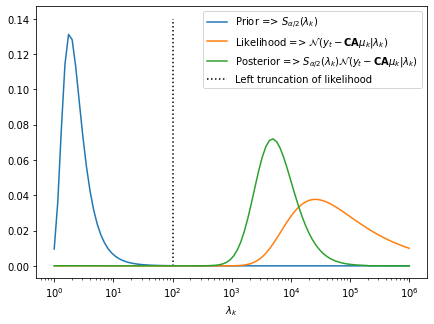
\includegraphics[width=12.0cm]{../plots/2__2__2__rejection_sampling_priors.png}
	\caption{Illustration of the poor acceptance rate regime of prior/likelihood interaction}
	\label{fig:2__2__2__rejection_sampling_priors}
\end{figure}

Due to the additional observation noise term ($d$), we are unable to use the Inverse Gamma approximation to the full posterior as detailed in \cite{godsill1999bayesian}. Instead, we attempt to improve the sampling efficiency by truncating the left tail of the likelihood distribution. 

Due to the intractability of calculating the Cumulative Distribution Function (CDF) of the likelihood analytically, we left-truncate the likelihood where it is smaller than a chosen epsilon. In this project, this small epsilon was chosen to be $\epsilon_{trunc} = 1 \times 10^{-50}$. Further checks are also performed to ensure that this truncation only occurs well into the right tail of the prior. 

This allows us to generate samples from a left-truncated form of the $\alpha$-stable prior instead of the full prior. These generated samples are much more likely to be in the high probability regions of the likelihood, thus improving our sampling efficiency greatly.

We sample from the left truncated \asd  by applying a paretian tail approximation to the \asd, then sampling from the paretian tail approximation using \autoref{eq:2__2__2__bounded_pareto}.

This improved rejection sampler can be described as:

\begin{enumerate}
	
	\item Define hyperparameter $\epsilon_{trunc}$
	\item Calculate 95th percentile of the prior ($\lambda_{0.95}$) where: $\int_{0}^{\lambda_{0.95}}\SAhalf(\lambda_k | 1,1,0) = 0.95$
	
	\item Draw proposals $\lambda_k^{(i)}$
	\begin{itemize}
		\item Calculate a possible truncation value $\lambda_{k, trunc}$ where $\mathcal{N}(\vt | \lambda_{k, trunc}) = \epsilon_{trunc}$.
		\item If this truncation value also lies in the right tail of the prior (i.e. $\lambda_{k, trunc} > \lambda_{0.95}$) then sample particle from the paretian tail approximation
		
		$$ \lambda_k^{(i)} \sim f_{bounded \text{ }pareto}(x | \alpha/2, \beta = 1, \lambda_{k, trunc}) $$
		
		\item Otherwise, sample particle from the original prior:
		
		$$ \lambda_k^{(i)} \sim \SAhalf(1,1,0) $$
	\end{itemize}
	
	\item Draw $ u \sim U ( 0, M )$
	\item If $u \geq \mathcal{N}\left( \vt | 0, \sigma_\lambda \lambda_k + \mu_\lambda \right)$, reject $\lambda_k^{(i)}$ and go to Step (3)
\end{enumerate}



%Next, we describe how to sample appropriately from the left truncated $\alpha$-stable distribution.
%
%We employ the tail approximation of the $\alpha$-stable distribution to a pareto distribution, noting that: 
%
%\begin{equation}
%	\lim_{\lambda_k \rightarrow \infty } S_{\alpha}(\lambda_k) \approx \alpha (1+\beta) C_\alpha \lambda_k^{-(1+\alpha)}
%\end{equation}
%
%Thus, up to a certain scale parameter($\alpha (1+\beta) C_\alpha$), sampling from the approximate left-truncated $\alpha$-stable distribution is equivalent to sampling from a left-truncated pareto distribution. 
%
%Lastly, we can sample from the appropriate left-truncated pareto distribution easily using the inverse transform method: 
%
%\begin{equation}
%	x = \left( \frac{1-(\frac{U}{\alpha (1+\beta) C_\alpha}) }{L^\alpha} \right) ^ {-\frac{1}{\alpha}}
%	\label{eq:2__2__2__bounded_pareto}
%\end{equation}
%
%Following \autoref{eq:2__2__2__bounded_pareto}, $x$ will be left-truncated $\alpha$-stable distributed if $U \sim \text{Unif}(0,1)$.

\end{document}